\documentclass[11pt]{article}
\usepackage[utf8]{inputenc} 
\usepackage[T1]{fontenc}
\usepackage{graphicx}
\usepackage[french]{babel}
\usepackage[in]{fullpage}

\usepackage{enumitem}
\usepackage{array}
\usepackage{multirow}

\usepackage{amsmath}
\usepackage{amssymb}
\usepackage{mathtools}

\usepackage{float}

\usepackage{pgf}
\usepackage{tikz}
\usepackage{tikzscale}
\usetikzlibrary{arrows,automata}
\usetikzlibrary{positioning}
\tikzset{
    rect/.style={
           rectangle,
           rounded corners,
           draw=black, very thick,
           minimum height=2em,
           inner sep=2pt,
           text centered,
           },
    circ/.style={
           circle,
           draw=black, very thick,
           minimum height=2em,
           inner sep=2pt,
           text centered,
           },
}

% Pour les cadres
\setlength{\fboxsep}{0.2cm} \newlength{\fboxwidth}
\addtolength{\fboxwidth}{4cm}
\addtolength{\fboxwidth}{\columnwidth} \addtolength{\fboxwidth}{-2 \fboxsep}
\addtolength{\fboxwidth}{-2 \fboxrule}
\newcommand{\parfbox}[1]{{\parindent0mm\fbox{\parbox{\fboxwidth}{#1}}}}

\newcommand{\R}{{\mathbb{R}}}

\DeclarePairedDelimiter\floor{\lfloor}{\rfloor}

\setlength{\parskip}{.2cm}

\begin{document}

%\everymath{\displaystyle}
\renewcommand\arraystretch{1.5}

{\parindent0mm
LINMA 1702 Mod\`{e}les et m\'{e}thodes d'optimisation \hfill Projet -- 2015 }
\begin{center} {\Large Planification de la production \\ d'une ligne d'assemblage de smartphones}

\bigskip

Groupe 15\\Pierre-Alexandre Louis, Simon Boigelot et Xavier Lambein
\end{center}

\section{Modélisation et implémentation \\de la ligne d'assemblage simple}

\parfbox{\textbf{Question 1.} Donnez une formulation linéaire (continue, sans variables entières) du problème de la planification de la ligne d'assemblage à personnel constant. Décrivez successivement variables, contraintes et fonction objectif. A ce stade, le fait de ne pas imposer l'intégralité des variables vous parait-il problématique ?}

\subsection*{Les variables et données du problème   }
Avant toutes choses, nous allons commencer par nommer et détailler les différentes données du problème. Celles-ci sont reprises dans la liste suivante:

\begin{itemize}[before={\renewcommand\makelabel[1]{\makebox[1cm][r]{##1\hspace{.2cm}}}}]
    \item[$T$] le nombre de semaines sur lesquelles on effectue la planification
    \item[$D^t$] la demande de smartphones pour la semaine $t$
    \item[$D_\mathrm{a}$] la durée d'assemblage d'un smartphone, en heures
    \item[$N_\mathrm{o}$] le nombre d'ouvriers
    \item[$N_\mathrm{h}$] le nombre d'heures normales disponibles pour assembler des smartphones, par semaine et par ouvrier
    \item[$N_\mathrm{hs}$] le nombre d'heures supplémentaires disponibles pour assembler des smartphones, par semaine et par ouvrier
    \item[$N_\mathrm{st}$] le nombre maximal de smartphones sous-traitables, par semaine 
    \item[$C_\mathrm{m}$] le coût des matériaux
    \item[$C_\mathrm{s}$] le coût du stockage d'un smartphone
    \item[$C_\mathrm{h}$] le coût horaire d'un ouvrier
    \item[$C_\mathrm{hs}$] le coût d'une heure supplémentaire de la part d'un ouvrier
    \item[$C_\mathrm{st}$] le coût de la sous-traitance pour l'assemblage d'un smartphone
    \item[$C_\mathrm{r}$] le coût supplémentaire associé au retard de livraison d'un smartphone
    \item[$C_\mathrm{e}$] le coût d'embauche d'un ouvrier
    \item[$C_\mathrm{l}$] le coût de licenciement d'un ouvrier
    \item[$S_\mathrm{i}$] le stock initial (et final) de smartphones
\end{itemize}

Viennent ensuite les variables:

\begin{itemize}[before={\renewcommand\makelabel[1]{\makebox[1cm][r]{##1\hspace{.2cm}}}}]
    \item[$n^t$] le nombre de smartphones produits en conditions normales
    \item[$n_\mathrm{hs}^t$] le nombre de smartphones produits en heures supplémentaires
    \item[$n_\mathrm{st}^t$] le nombre de smartphones produits en sous-traitance
    \item[$s^0$] le stock initial de smartphones
    \item[$s^t$] le stock de smartphones à la fin de la semaine $t$, disponible en semaine $t+1$, pour lequel on paye le stockage en semaine $t$
    \item[$r^t$] les smartphones retardés lors de la semaine $t-1$, à produire et livrer en semaine $t$
\end{itemize}

\subsection*{Les contraintes}

Ceci fait, nous pouvons maintenant lister les contraintes selon lesquelles nous allons optimiser:

\begin{enumerate}
    \item égalité entre
    \begin{itemize}
        \item les smartphones produits et disponible en stock en début de semaine et
        \item la demande, le stock disponible en fin de semaine et le retard de la semaine passé, moins le retard que l'on décide de prendre cette semaine :
    \end{itemize}
    \[
        n^t + n_\mathrm{hs}^t + n_\mathrm{st}^t + s^{t-1} = D^t + s^t + r^t - r^{t+1}
        \text;
    \]
    
    \item nécessité de produire chaque semaine au moins le nombre de smartphones retardés lors de la semaine précédente (afin de ne pas avoir un retard de deux semaines) :
    \[
        n^t + n_\mathrm{hs}^t + n_\mathrm{st}^t + (s^{t-1} - s^t) \geq r^t
        \text;
    \]
    
    \item limite sur la capacité en heures normales, supplémentaires et en sous-traitance :
    \[
        n^t \leq \frac{N_\mathrm{h}\,N_\mathrm{o}}{D_\mathrm{a}}
        \text,\qquad
        n_\mathrm{hs}^t \leq \frac{N_\mathrm{hs}\,N_\mathrm{o}}{D_\mathrm{a}}
        \quad\text{et}\quad
        n_\mathrm{st}^t \leq N_\mathrm{st}
        \text;
    \]
    
    \item stock initial et final fixé à $S_\mathrm{i}$ :
    \[
        s^0 = S_\mathrm{i} \quad\text{et}\quad s^T = S_\mathrm{i}
        \text;
    \]
    
    \item pas de retard à rattrapper en semaine 1 :
    \[
        r^1 = 0
        \text{;}
    \]
    
    \item enfin, toutes les variables positives :
    \[
        n^t, n_\mathrm{hs}^t, n_\mathrm{st}^t, s^t, s^T, r^t, r^T \geq 0
        \text;
    \]
\end{enumerate}

\subsection*{La fonction objectif}

Terminons par la fonction objectif. Soit
$f(x) : \mathbb{R}^{5T+1} \rightarrow \mathbb{R}$,
avec $x$ un vecteur de $\mathbb{R}^{5T+1}$:
\[
    x = (n^1,\dots,n^T,n_\mathrm{hs}^1,\dots,n_\mathrm{hs}^T,n_\mathrm{st}^1,\dots,n_\mathrm{st}^T,s^0,\dots,s^T,r^1,\dots,r^T)
    \text.
\]

Par simplicité, nous allons décomposer $f(x)$ en une somme de fonctions $f^t$ définies pour chaque semaine $t$:
\[
    f(x) = \sum_{t=1}^{T} f^t(n^t, n_\mathrm{hs}^t, n_\mathrm{st}^t, s^t, r^t)
\]
et
\begin{align*}
    f^t(n^t, n_\mathrm{hs}^t, n_\mathrm{st}^t, s^t, r^t)
    &= (n^t + n_\mathrm{hs}^t)\,C_\mathrm{m} 
    & \text{prix des matériaux}\\
    &+ n_\mathrm{hs}^t\,D_\mathrm{a}\,C_\mathrm{hs}
    & \text{production en heures supplémentaires}\\
    &+ n_\mathrm{st}^t\,C_\mathrm{st}
    & \text{production sous-traitée}\\
    &+ s^t\,C_\mathrm{s}
    & \text{stockage des smartphones}\\
    &+ r^t\,C_\mathrm{r}
    & \text{retard de livraison}
    \text.
\end{align*}

Il est à noter que le salaire en heure normale des ouvriers n'apparaît pas dans cette fonction: nous ne sommes plus au XIXe siècle, un ouvrier est donc toujours payé pour sa semaine, peu importe le travail qu'il a réellement effectué. Il s'agit donc d'un coût fixe que l'on ne peut pas optimiser sans licencier des ouvriers.

\subsection*{Le modèle complet}

En résumé, le problème se modélise de la manière suivante :
\begin{align*}
    \min_{x}\;f(x) =& \sum_{t=1}^{T}
    (n^t + n_\mathrm{hs}^t)\,C_\mathrm{m} 
    + n_\mathrm{hs}^t\,D_\mathrm{a}\,C_\mathrm{hs} \\
    &+ n_\mathrm{st}^t\,C_\mathrm{st}
    + s^t\,C_\mathrm{s}
    + r^t\,C_\mathrm{r} \\[0.5em]
%
    \mathrm{s.c.q.}\;\phantom{f(x) =}
    & n^t + n_\mathrm{hs}^t + n_\mathrm{st}^t + s^{t-1} = D^t + s^t + r^t - r^{t+1} \\
    & n^t + n_\mathrm{hs}^t + n_\mathrm{st}^t + (s^{t-1} - s^t) \geq r^t \\
    & n^t \leq N_\mathrm{h}\,N_\mathrm{o}/D_\mathrm{a} \\
    & n_\mathrm{hs}^t \leq N_\mathrm{hs}\,N_\mathrm{o}/D_\mathrm{a} \\
    & n_\mathrm{st}^t \leq N_\mathrm{st} \\
    & s^0 = S_\mathrm{i} \\
    & s^T = S_\mathrm{i} \\
    & r^1 = 0 \\
    & n^t, n_\mathrm{hs}^t, n_\mathrm{st}^t, s^t, s^T, r^t, r^T \geq 0 \\
\end{align*}

À ce stade-ci, on peut se demander si l'hypothèse des variables non-entières n'entraînera pas des résultats aberrants, tel qu'un nombre de smartphones produits non-entier.


%\emph{Vous pouvez utiliser des notations mathématiques classiques pour décrires vos variables, fonction, contraintes. Il est conseillé de leur donner des noms mémorables (p.ex. variable $qp_t$ pour une quantité produite au temps $t$, plutôt que $x_i$). Il n'est pas nécessaire de décrire les matrices/vecteurs "fusionnés" $A$, $b$, $c$ qui seront assemblés et fournis au solver MATLAB à la question 3.}


\parfbox{\textbf{Question 2.} Démontrez que, sous certaines hypothèses raisonnables, il est possible de garantir que votre modèle linéaire continu admette toujours une solution entière, c'est-à-dire ne comportant que des quantités produites entières chaque semaine. L'une de ces hypothèses est l'intégralité de la demande chaque semaine ; quelles sont les autres ?}

Afin de montrer que le problème relaxé donne une solution entière, nous allons montrer que le problème peut être reformulé sous la forme d'un flot de coût minimal, dont les capacités et les entrées/sorties sont entières.

Voici comment nous avons reformulé le problème : nous avons défini un graphe orienté dont les deux noeuds d'entrée ont pour valeur $D=\sum_{i=0}^{T-1} D^t$, c'est-à-dire la quantité de smartphones à produire au total, et $s^0 = S_\mathrm{i}$, c'est-à-dire le stock initial de smartphones.

Le graphe possède $T+1$ sorties, qui sont les demandes de chaque semaine $D^t$, et le stock de la dernière semaine $s^T = S_\mathrm{i}$. On note que la somme des entrées est égale à la somme des sorties, ce qui doit être le cas dans un problème de flot.

Le flot d'entrée $D$ va parcourir le graphe à travers $3T$ arrêtes sortantes de \og{}production\fg{}, correspondantes aux variables $n^t$, $n_\mathrm{hs}^t$, $n_\mathrm{st}^t$ pour chaque semaine $t \in \{1,\dots,T\}$. Celles-ci ont des coûts et des capacités correspondant à la variable associée, c'est-à-dire:
\begin{center}
\begin{tabular}{c|cc}
    \textbf{Variable} & \textbf{Coût} & \textbf{Capacité} \\
    \hline
    $n^t$ & $C_\mathrm{m}$ & $N_\mathrm{h}\,N_\mathrm{o}/D_\mathrm{a}$ \\
    \hline
    $n_\mathrm{hs}^t$ & $C_\mathrm{m}+C_\mathrm{hs}/D_\mathrm{a}$ & $N_\mathrm{hs}\,N_\mathrm{o}/D_\mathrm{a}$ \\
    \hline
    $n_\mathrm{st}^t$ & $C_\mathrm{st}$ & $N_\mathrm{st}$ \\
\end{tabular}
\end{center}

Par simplicité, nous regroupons toute la production d'une semaine dans un noeud $P^t$. À partir de celui-ci, la production est redistribuée par des arêtes sortantes dans trois autres noeuds: la demande de cette semaine $D^t$, le stock de cette semaine $s^t$ et la demande de la semaine passée $D^{t-1}$.

La première arête correspond simplement à remplire la demande de la semaine actuelle avec la production de cette même semaine, et a donc un coup nul et une capacité infinie: en effet, le prix de fabrication a déjà été payé avant d'arriver au noeud $P^t$, et la capacité est implicite, car le noeud de demande va être rempli jusqu'à-ce-que son entrée soit égale à sa sortie, qui vaut $D^t$.

La seconde arête correspond à la production étant mise de côté dans le stock $s^t$. Celle-ci possède un coût, qui est celui de stockage $C_s$, et une capacité infinie, car il n'y a pas de contrainte sur la taille du stock.

Enfin, la troisième arrête correspond à la production en retard, qui est envoyée à la demande de la semaine précédente. Elle a donc un coût $C_r$ et une capacité infinie.

Pour terminer, les noeuds de stock $s^t$ possèdent chacun deux arêtes sortantes. La première est connectée à la demande de la semaine suivante $D^{t+1}$, sans coût car celui-ci a déjà été payé, et possède avec une capacité infinie. La seconde est connectée au stock de la semaine suivante $s^{t+1}$, avec un coût qui est celui de stockage $C_s$ et une capacité infinie.

Les différentes arêtes sont reprises dans le tableau suivant:
\begin{center}
\begin{tabular}{cc|c|cc|c}
    \textbf{De} & \textbf{À} & \textbf{Variable} & \textbf{Coût} & \textbf{Capacité} & $\forall t \in$ \\
    \hline
    $D$ & $P^t$ &
    $n^t$ & $C_\mathrm{m}$ & $N_\mathrm{h}\,N_\mathrm{o}/D_\mathrm{a}$
    & $1,\dots,T$ \\
    \hline
    $D$ & $P^t$ &
    $n_\mathrm{hs}^t$ & $C_\mathrm{m}+C_\mathrm{hs}/D_\mathrm{a}$ & $N_\mathrm{hs}\,N_\mathrm{o}/D_\mathrm{a}$
    & $1,\dots,T$ \\
    \hline
    $D$ & $P^t$ &
    $n_\mathrm{st}^t$ & $C_\mathrm{st}$ & $N_\mathrm{st}$
    & $1,\dots,T$ \\
    
    \hline
    $P^t$ & $D^t$ &
    --- & $0$ & $\infty$
    & $1,\dots,T$ \\
    \hline
    $P^t$ & $s^t$ &
    $s^t$\;\underline{*} & $C_\mathrm{s}$ & $\infty$
    & $1,\dots,T$ \\
    \hline
    $P^t$ & $D^{t-1}$ &
    $r^t$ & $C_\mathrm{r}$ & $\infty$
    & $2,\dots,T$ \\
    
    \hline
    $s^t$ & $D^{t+1}$ &
    --- & $0$ & $\infty$
    & $1,\dots,T-1$ \\
    \hline
    $s^t$ & $s^{t+1}$ &
    $s^t$\;\underline{*} & $C_\mathrm{s}$ & $\infty$
    & $1,\dots,T-1$ \\
\end{tabular}
\end{center}

Il est à noter que $s^t$ ne correspond pas directement à une arête; au lieu de cela, la variable correspond à la somme des entrées sur le noeud $s^t$, c'est-à-dire à la somme des deux arêtes dont la variable est intitulée \og{}$s^t$\;\underline{*}\fg{} dans le tableau.

Un schéma de ce graphe est représenté dans la figure~\ref{fig:q2_flow}.

Maintenant que le graphe a été construit, le théorème sur les flots de coût minimum nous indique que si les demandes et les capacités du graphe sont entières, alors il existe une solution optimale entière au flot de coût minimum, et donc au problème de la question 1, les deux étant équivalents.

Imposer que les demandes et capacités soient entières revient à imposer que les grandeurs suivantes soient entières:
\begin{itemize}
    \item $D^t \forall t \in 1,\dots,T$, ce qui est le cas: il s'agit d'un nombre de smartphones;
    \item $s^0$ et $s^T$, ce qui est également le cas, pour la même raison;
    \item $N_\mathrm{st}$, qui, de nouveau, est un nombre de smartphones;
    \item $N_\mathrm{h}\,N_\mathrm{o}/D_\mathrm{a}$ et $N_\mathrm{hs}\,N_\mathrm{o}/D_\mathrm{a}$, qui sont entiers si le numérateur est multiple du dénominateur, ou bien si l'on impose l'hypothèse tout à fait raisonnable d'arrondir cette valeur à l'entier inférieur.
\end{itemize}

Les conditions sont donc bien vérifiées pour avoir un problème relaxé avec une solution entière, à condition de remplacer $N_\mathrm{h}\,N_\mathrm{o}/D_\mathrm{a}$ par $\floor{N_\mathrm{h}\,N_\mathrm{o}/D_\mathrm{a}}$, et similairement pour $N_\mathrm{hs}$.

\begin{figure}[H]
    \centering
    \scalebox{1}{\includegraphics{q2_flow1.tikz}}
    \scalebox{1}{\includegraphics{q2_flow2.tikz}}
    \scalebox{1}{\includegraphics{q2_flow3.tikz}}
    \caption{Graphes orientés représentant la première, la $t$-ème et la dernière semaine. Les entrées et sorties sont en rectangle, et les autres noeuds sont en cercle. Dans chaque noeud est indiqué la variable correspondante, avec un signe négatif dans le cas des sorties. Dans le cas des noeuds normaux, la variable correspond à la somme des flots des arêtes entrantes. Les variables indiquées à côté de certaines arêtes correspondent au flot qui passe dans ces arêtes. Les arrêtes en pointillés indiquent un plus grand nombre d'arrêtes, qui n'ont pas été représentées par simplicité. De même, les points de suspension indiquent qu'il manque le reste du graphe (c'est-à-dire, les autres semaines).}
    \label{fig:q2_flow}
\end{figure}


%\emph{On attend ici une véritable preuve mathématique, qui peut faire appel à des résultats vus au cours. L'inclusion d'un schéma pourrait s'avérer utile.}

\parfbox{\textbf{Question 3.} Implémentez sous MATLAB ce modèle linéaire continu, et calculez la solution correspondant aux données fournies sur icampus (utilisez la fonction \texttt{linprog}). Commentez l'allure de la solution obtenue.}

La résolution du problème via Matlab nous montre que, lorsque le nombre d'ouvriers est constant, l'usine tourne à plein régime en permanence, accumule beaucoup de stock et de retard, jusqu'à parfois devoir recourir à la sous-traitance pour livrer dans les temps.

Il semble évident qu'un important bottleneck se situe au niveau du nombre d'ouviers disponibles, d'où l'ajout, à partir de la question 7, du nombre variable d'ouviers.

On notera que la fonction coût diffère d'une constante entre le rapport le programme Matlab; en effet, dans ce dernier, la fonction tient compte du coût horaire du travail de tous les employés sur les différentes semaines. Ce simple ajout permet d'avoir le coût réel de la production.

\begin{figure}[h]
    \centering
    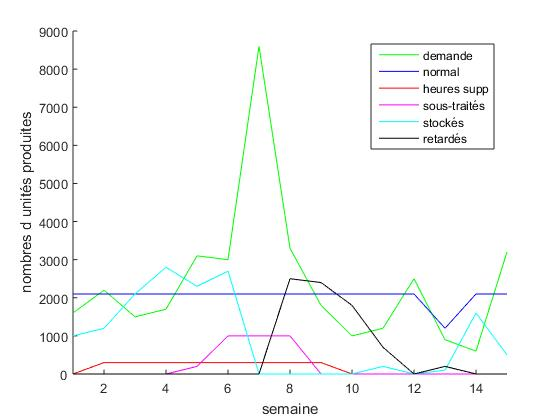
\includegraphics[width=0.8\textwidth]{graphes/graphq3.jpg}
    \caption{Graphe de la production à personnel constant}
    \label{fig:q3}
\end{figure}


%\emph{Il est inutile d'inclure ici vos codes MATLAB (ceux-ci seront transmis via icampus). Vous pouvez tout au plus commenter l'un ou l'autre aspect particulier de votre programme, si vous le jugez utile. La partie commentaire est la plus importante (elle peut inclure quelques observations sur le comportement du solver \texttt{linprog}).}

%\emph{Conseils pour la rédaction des codes MATLAB : essayez autant que possible que votre code fonctionne directement à l'aide des données fournies en argument (son exécution pourrait par exemple correspondre à la commande \texttt{solution = modelesimpleq3(donnees)}, où la structure \texttt{solution} contiendra toutes les données utiles calculées par votre code). Vous pouvez créer une fonction (ou un script) différente pour chaque question qui nécessite une implémentation MATLAB. Si vous incluez des figures MATLAB dans votre rapport, vous pouvez également joindre le code qui a produit ces figures.}


\parfbox{\textbf{Question 4.} Décrivez une procédure permettant, avec le moins de nouveaux calculs possibles, d'évaluer les conséquences sur la fonction objectif d’une petite variation de la demande prévue. Plus précisément, analysez l'effet du remplacement du vecteur \texttt{demande} par le vecteur \texttt{demande + epsilon * delta\textunderscore demande} où \texttt{delta\textunderscore demande} est un vecteur de perturbation sur la demande, et \texttt{epsilon} est un paramètre scalaire dont la valeur est faible.}

Tout problème d'optimisation linéaire possède un problème companion, appelé problème dual, pour lequel le rôle des variables et des contraintes est inversé. A chaque variable dans le primal est associée une contrainte dans le dual est vice-versa.

Dans notre cas, le problème primal nous permet de connaître quelles quantités de smartphone nous devons produire et dans quel timing afin de diminuer un maximum nos dépenses et, infine, augmenter notre profit. Et ce en considérant nos ressources comme fixes.

Si nous désirons observer ce que nous pourrions obtenir avec une quantité en plus d'une certaine ressource, nous devons connaître la sensibilté du primal vis-à-vis de cette même ressource. C'est le rôle du dual. Il nous donne l'influence ou le prix des variables. Soit un problème d'optimisation linéaire sous forme standard:
\[
    \min_{x}\,c^{T}x
    \quad\text{tel que}\quad
    Ax = b
    \quad\text{avec}\quad
    x \geq 0
\]

Nous pouvons y associer le problème dual suivant:
\[
    \max_{y}\,b^{T}y
    \quad\text{tel que}\quad
    A^{T}y = c
    \quad\text{avec}\quad
    y \text{ libre}
\]

Considérons la solution optimale de ces deux problèmes comme étant respectivement $x^{*}$ et $y^{*}$. Par la dualité forte et puisque nous sommes en présence d'un problème linéaire, nous avons d'office $ c^{T}x^{*} = b^{T}y^{*}$

Si le vecteur des ressources devient $ b' = b + \Delta b $. $\Delta b$ ne doit pas être trop grand afin que la base optimale du problème ne change pas au sinon. En effet, cela corresprondrait à "sauter" sur un autre sommet du polyèdre et donnerait donc des résultats totalement différents. Supposons doc cette contrainte satisfaite, la fonction objectif du problème primal sera alors incréméntée d'une quantité $y^{*^{T}}\Delta b$. Dans notre cas, après avoir calculé la solution du primal avec le vecteur \textbf{demande} et après avoir calculé la solution du dual une fois pour toute, il ne faudra plus que rajouter $y^{*^{T}} \cdot \textbf{epsilon * delta\_demande}$.


%\emph{Seule une réponse théorique est demandée à ce stade.}


\parfbox{\textbf{Question 5.} Testez sous MATLAB la procédure du point précédent avec les données fournies. Comparez ensuite la prédiction obtenue par cette procédure avec la valeur obtenue en résolvant à nouveau complètement le modèle, et ce pour un échantillon de valeurs du paramètre \texttt{epsilon} comprises entre $0$ et $1$ (par exemple \texttt{0:.1:1}). Commentez (éventuellement en vous aidant d'un graphique).}

Ci-dessous, un graphe qui montre la différence entre le coût obtenu, pour un certain epsilon et pour une certaine légère modification de la demande, via la procédure présentée à la question 4 et le coût obtenu en résolvant complètement le problème avec les données initiales modifiées. Sur le graphe la différence est normalisée en pourcentage par rapport au résultat obtenu via la seconde méthode. Chaque point vaut:
\begin{equation*}
difference = \frac{resultat_{dual} - resultat_{reecriture}}{résultat_{reecriture}} * 100 
\end{equation*}
 
\begin{figure}[h]
    \centering
    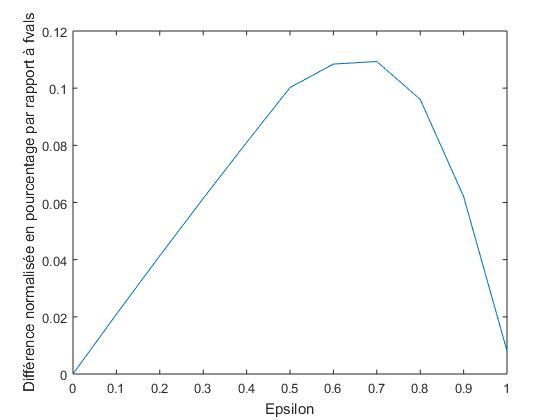
\includegraphics[width=0.8\textwidth]{graphes/graphq5.jpg}
    \caption{Graphe de la production à personnel constant}
    \label{fig:q5}
\end{figure}

La différence entre les deux méthodes dépasse à peine les 0,1\%. C'est négligeable à l'échelle utilisée ici. La procédure présentée à la question 4 est donc suffisante.

%\emph{A nouveau il n'est pas nécessaire d'inclure ici les quelques lignes de code nécessaires à ces calculs, mais bien sur icampus. Comparaison et commentaires sont les plus importants.}


\parfbox{\textbf{Question 6.} Décrivez (sans l'implémenter) l'adaptation qu'il serait nécessaire à apporter au modèle si le coût de l'heure supplémentaire pris en compte était variable. Plus concrètement, considérez qu'après la première heure supplémentaire (facturée au coût horaire \texttt{cout\textunderscore heure\textunderscore sup} standard), chaque heure supplémentaire (éventuellement) est facturée à un coût horaire supérieur de $5 \%$ à celui de l'heure supplémentaire précédente. Est-il toujours possible de formuler (ou reformuler) le problème sous forme linéaire ? Expliquez. Et que se passerait-il si le coût horaire des supplémentaires \emph{diminuait}  lorsque le nombre d'heure prestées augmente ? Justifiez.}

Le coût variable pour les heures supplémentaires modifie radicalement le problème, le rendant non-linéaire. En effet, si on considère $C$ le coût d'une heure supplémentaire et $n$ le nombre d'heures supplémentaires, avec un taux d'augmentation de $5\%$, le coût total des heures supplémentaires $C_\text{tot}$ est le suivant:
\begin{align*}
    C_\text{tot}
    &= C + C (105\%) + C (105\%)^2 + \dots + C (105\%)^{n-1}
    &= \sum_{i=0}^{n-1} C (105\%)^i
    \text.
\end{align*}
Nous voyons aisément, parce-que $n$ apparaît en exposant, que $C_\text{tot}$ n'est plus linéaire selon cette variable.

Le problème complet se présente donc de la manière suivante :
\[
    \text{min}_{\dots,n,\dots} f(\dots,n,\dots) = \dots + C_\text{tot} + \dots
    \text.
\]
Le reste de la fonction objectif ne changeant pas, nous l'avons omis. Seul $C_\text{tot}$ est différent. Comme celui-ci n'est plus linéaire, $f$ n'est plus non plus linéaire selon l'une des variables par rapports auxquelles on optimise. Le problème n'est donc plus linéaire.

La même situation apparaît si l'on voulait diminuer le coût des heures supplémentaires: il suffit de remplacer $105\%$ par une valeur inférieure à $100\%$. On obtiendra une exponentielle décroissante, qui n'est bien évidemment toujours pas linéaire.


%\emph{Seule une réponse théorique est demandée. Réutilisez autant que possible les éléments inchangés (variables, contraintes, etc.) du modèle de la Question 1.}


\section{Modélisation et implémentation \\de la ligne d'assemblage avec gestion du personnel}

\parfbox{\textbf{Question 7.} Donnez à présent une formulation linéaire (continue, sans variables entières) du problème de la planification de la ligne d'assemblage incluant le gestion du personnel, en vous basant sur le modèle déjà construit à la Question 1. Décrivez successivement variables, contraintes et fonction objectif.}

Afin d'inclure la variation du nombre d'employés, nous introduisons trois nouvelles variables pour chaque semaine: $n_\text{o}^t$, le nombre d'ouvriers après embauche et licenciement, $n_\text{e}^t$ le nombre d'embauches et $n_\text{l}^t$, le nombre de licenciements.

De nouvelles contraintes sur ces variables sont ajoutées:
\begin{enumerate}
    \item nouvelles variables positives:
    \[
        n_\text{o}^t, n_\text{e}^t, n_\text{l}^t \geq 0
        \text;
    \]
    
    \item la variation du nombre d'ouvrier doit dépendre du nombre d'embauche et de licenciement:
    \[
        n_\text{o}^t - n_\text{o}^{t-1} = n_\text{e}^t - n_\text{l}^t
        \text;
    \]
    
    \item les limites sur la capacité en heures normales et supplémentaires changent pour dépendre du nombre d'ouvriers :
    \[
        n_hs^t \leq N_{hs,max}
        \text.
    \]
\end{enumerate}

Enfin, la fonction-objectif est modifiée pour inclure:
\begin{itemize}
    \item le salaire des ouvriers, qui n'est plus constant:
    \[
        n_\text{o}^t*C_\text{o}
        \text{ et }
    \]
    
    \item le prix d'embauche et de licenciement:
    \[
        n_\text{e}^t*C_\text{e} + n_\text{l}^t*C_\text{l}
        \text.
    \]
\end{itemize}


%\emph{Cf. instructions de la Question 1. Réutilisez autant que possible les éléments inchangés (variables, contraintes, etc.).}

\parfbox{\textbf{Question 8.} Implémentez sous MATLAB ce modèle linéaire continu, et calculez la solution correspondant aux données fournies sur icampus. Commentez l'allure de la solution obtenue, et comparez à la solution du modèle simplifié. Commentez également l'intégralité des variables de la solution ; celle-ci présente-t-elle un aspect problématique ?}

En optimisant également le nombre d'ouvriers, nous obtenons un graphe qui suit beaucoup mieux la courbe de demande: l'usine tourne toujours au maximum, mais en adaptant son nombre d'ouvriers. Il y a moins de stock, largement moins d'heures supplémentaires, et la sous-traitance a même totalement disparu.

Cependant, puisque l'on n'a pas imposé l'intégralité des variables, nous obtenons un nombre d'ouvriers non-entier, ce qui n'est pas possible en réalité.

\begin{figure}[H]
    \centering
    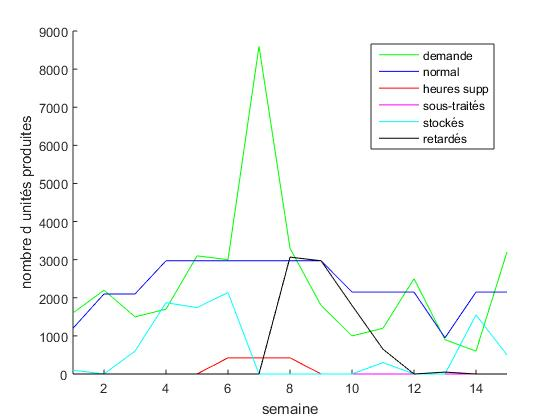
\includegraphics[width=0.8\textwidth]{graphes/graphq8.jpg}
    \caption{Graphe de la production à personnel variable non-entier}
    \label{fig:q8_01}
\end{figure}

\begin{figure}[H]
    \centering
    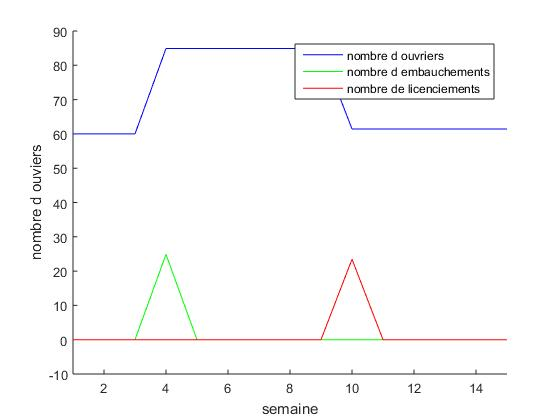
\includegraphics[width=0.8\textwidth]{graphes/ouvrierq8.jpg}
    \caption{Graphe de la variation du personnel non-entier}
    \label{fig:q8_02}
\end{figure}


%\emph{Cf. instructions de la Question 3.}

\parfbox{\textbf{Question 9.} Résolvez à nouveau ce modèle en imposant à présent l'intégralité des variables pour lesquelles c'est absolument indispensable (utilisez la fonction \texttt{intlinprog}). Commentez l'allure de la solution obtenue, et comparez aux solutions obtenues précédemment.}

Ici, nous avons ajouté l'hypothèse des variables entières dans le solveur, ce qui a pour effet de modifier légèrement la courbe, tout en gardant les caractéristiques importantes observées à la question précédente.

\begin{figure}[H]
    \centering
    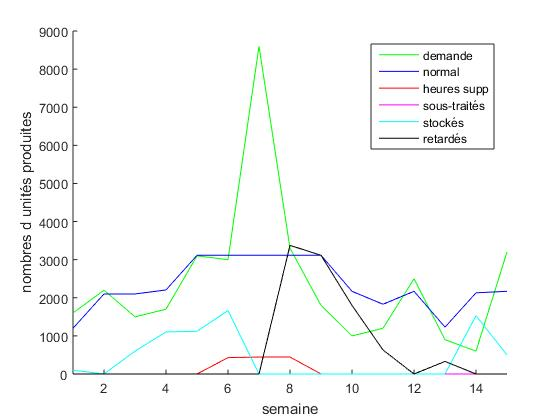
\includegraphics[width=0.8\textwidth]{graphes/graphq9.jpg}
    \caption{Graphe de la production à personnel variable entier}
    \label{fig:q8_01}
\end{figure}

\begin{figure}[H]
    \centering
    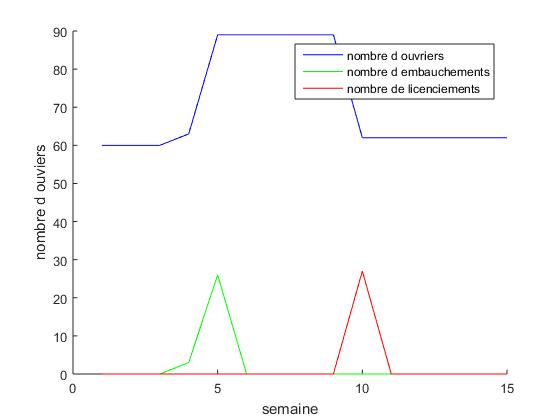
\includegraphics[width=0.8\textwidth]{graphes/ouvrierq9.jpg}
    \caption{Graphe de la variation du personnel entier}
    \label{fig:q8_02}
\end{figure}


%\emph{Cf. instructions de la Question 3.}


\section{Critique}
\parfbox{\textbf{Question 10.} Critiquez les modèles proposés dans ce projet. Sont-ils réalistes ? Des approximations ont-elles été faites et, si oui sont-elles justifiées ? Quelles améliorations pourriez-vous proposer (sans rentrer dans les détails), avec quel impact potentiel sur la résolution du problème.}

Plusieurs critiques peuvent être émises sur la modélisation.

Tout d'abord, parlons de  l'embauche. Bien que le modèle prenne en compte un coût d'embauche pour chaque nouvel employé, il oublie le fait qu'un nouveau ouvrier travaille moins bien qu'un ouvrier expérimenté. Il prendra, à priori, plus de temps pour assembler un smartphone. Afin de combler ce manque, il serait utile d'ajouté un type de variables, le nombre de nouveaux ouvriers engagés lors d'une semaine, et un paramètre, la durée d'assemblage pour des nouveaux ouvriers . Ainsi, une personne engagée en semaine \textit{T}, sera durant un certain nombre de semaines \textit{Nb} capable de produire des produits à une durée d'assemblage \textit{D-a-nouveau} et elle sera ajoutée au nombre de nouveau employés. Le nombre d'ouvriers restera constant. Après \textit{Nb} semaines, l'ouvrier est placé dans les ouvriers classiques. Le nombre de nouveaux ouvriers diminue de 1 et celui des ouvriers normaux augmente de 1.

Le modèle ne prend pas en compte les jours fériés légaux qui peuvent survenir pendant les semaines sur lesquelles est établie l'optimisation. Ceci  amène une perte de précision et une diminution du coût réel. En effet, si les ouvriers ne peuvent travailler un jour férié légal, il sera peut-être obligatoire d'engager plus de personnel pour répondre à la demande ou de sous-traiter une plus grande quantité de produit. Pour pallier ce problème, il faudrait passer en paramètre le nombre de jour férié présent dans chacune des semaines de planification. Notons néanmoins que si l'usine est localisée en Chine, ce problème ne se posera jamais.

%\emph{C'est ici que vous pouvez, si vous le souhaitez, prendre un peu de recul par rapport à ce qui vous était demandé, et exercer votre esprit critique.}

\end{document}
